\subsection{LDAP Account Manager}

Esta interface permite ao administrador gerir os utilizadores nas tarefas mais comuns como criar, editar ou remover utilizadores.
Todos os dados dos utilizadores estão num directório LDAP que pode ser acedido via browser:
\begin{description}
	\item[endereço:] \lamurl
	\item[password:] \lampassword
\end{description}

Irá encontrar a seguinte página:

\begin{figure}[H]
    \begin{center}
        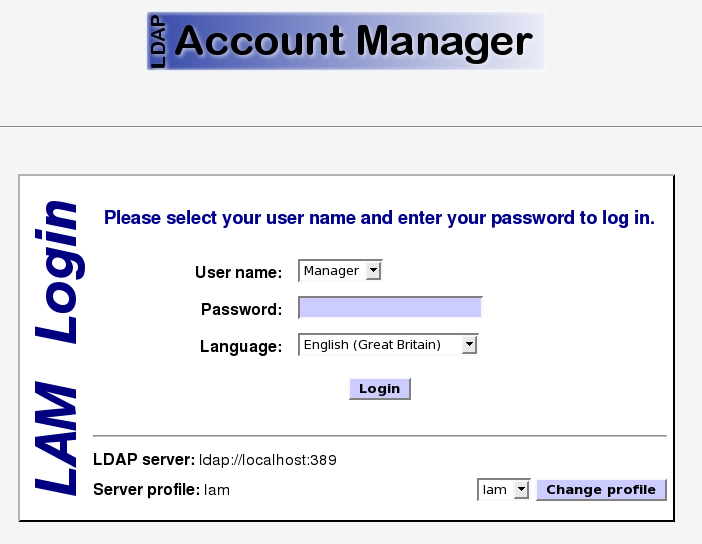
\includegraphics[width=10cm]{include/img/lam1}
    \end{center}
    \caption{Página inicial do LAM}
    \label{fig:LAM1}
\end{figure}


Após inserir a palavra-passe correcta e carregar no botão de Login deverá ir ter à seguinte página:

\begin{figure}[H]
    \begin{center}
        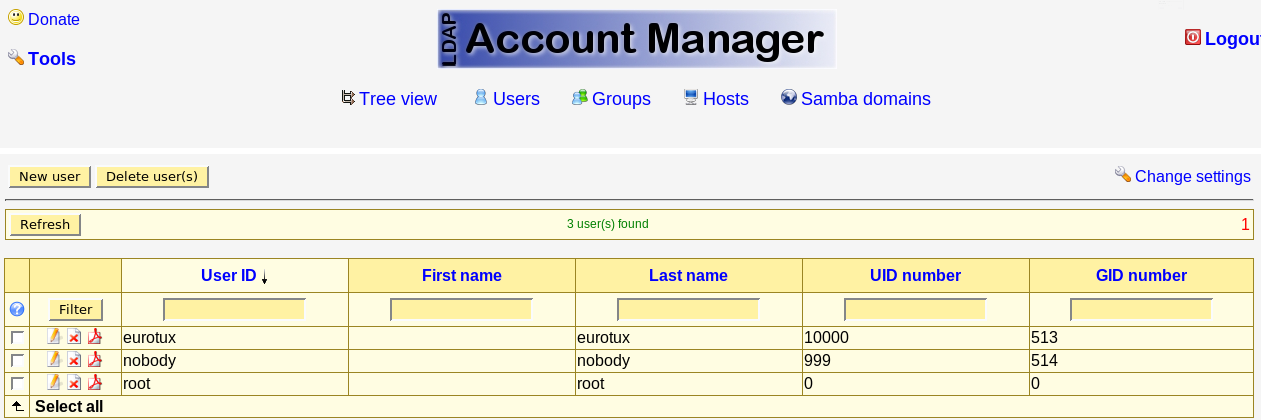
\includegraphics[width=10cm]{include/img/lam2}
    \end{center}
    \caption{Menu LAM}
    \label{fig:LAM2}
\end{figure}

Como poderá verificar, já existem três utilizadores criados, o "root", o "eurotux" e o "nobody". No menu superior encontra os seguintes items:

\begin{itemize}
\item Tree View - Permite ver sob a forma de árvore o conteúdo da base de dados LDAP
\item Users - Apresenta a listagem de utilizadores
\item Groups - Apresenta a listagem dos grupos de utilizadores
\item Hosts - Apresenta a listagem dos postos ligados ao domínio SAMBA
\item Samba domains - Apresenta os domínios samba
\end{itemize}

\subsubsection{Tree View}
Quando o utilizador carrega nesta ligação vai-lhe ser ser apresentada a listagem visual da árvore LDAP. Podemos então verificar que na raíz da árvore LDAP estão visíveis as unidades organizativas de computadores, domínios, grupos e utilizadores. Caso o cliente tenha adquirido o módulo de lista de endereços partilhada também estará visível a lista de endereços.

\begin{figure}[H]
    \begin{center}
        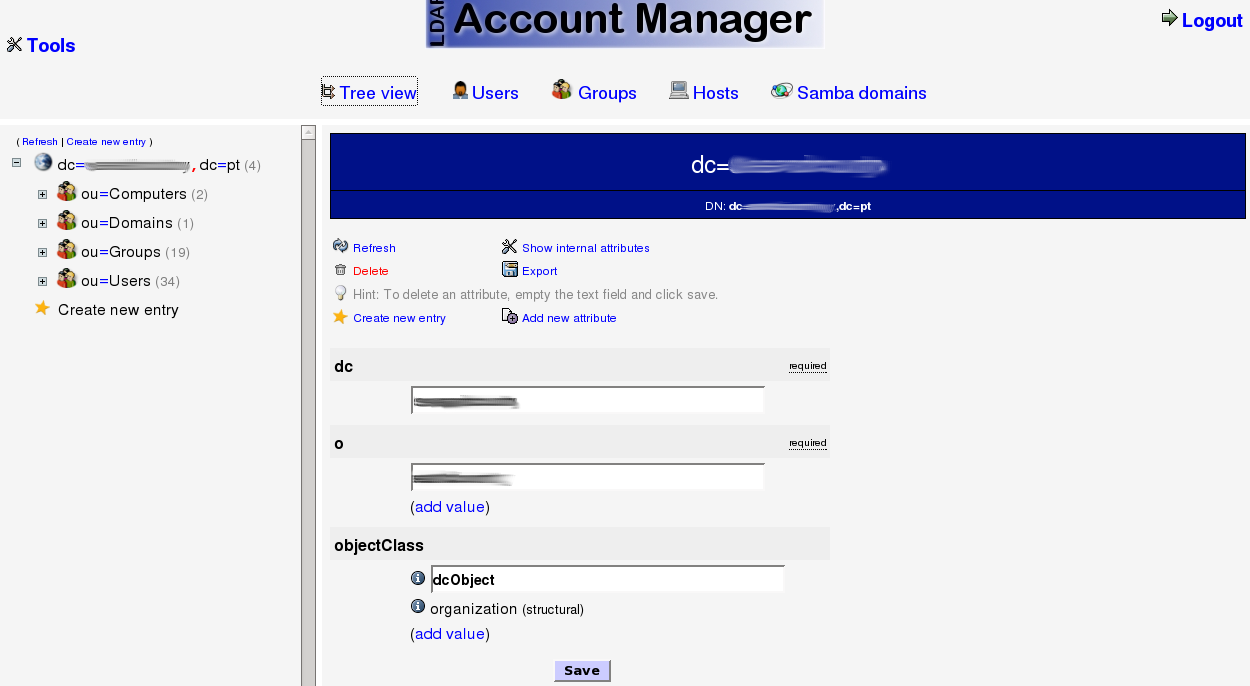
\includegraphics[width=10cm]{include/img/lam3}
    \end{center}
    \caption{Esquema em árvore}
    \label{fig:LAM3}
\end{figure}

Neste interface poderá navegar pela árvore LDAP e efectuar alterações ao nível dos atributos dos objectos da árvore. Como são alterações a baixo nível, não aconselhamos ao utilizador iniciado que efectue alterações nesta interface.

\subsubsection{Users}

A página que lhe será apresentada quando carregar nesta ligação será a seguinte:

\begin{figure}[H]
    \begin{center}
        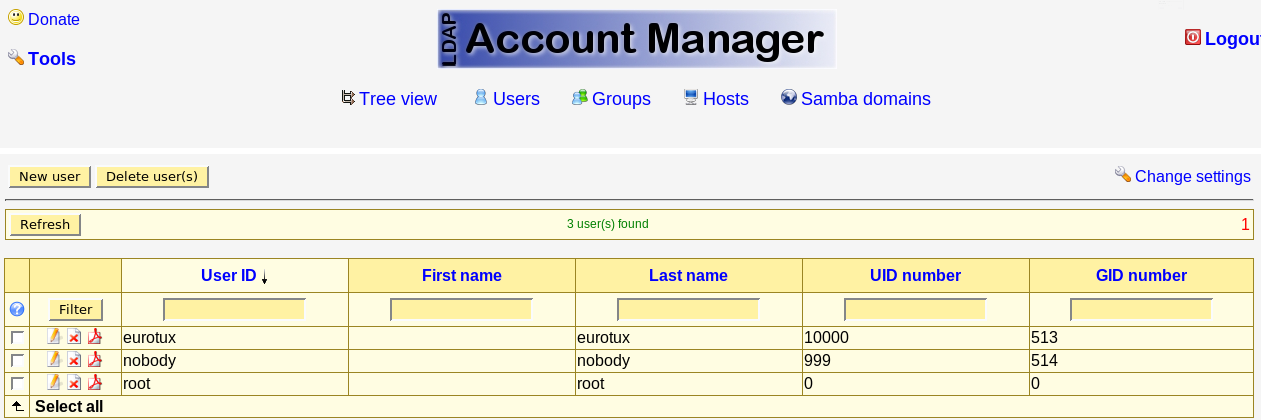
\includegraphics[width=10cm]{include/img/lam2}
    \end{center}
    \caption{Listagem Utilizadores}
    \label{fig:LAM2}
\end{figure}

Para editar um utilizador deverá carregar sobre o ícone "Edit" correspondente ao mesmo. Ser-lhe-á apresentada a seguinte página:

\begin{figure}[H]
    \begin{center}
        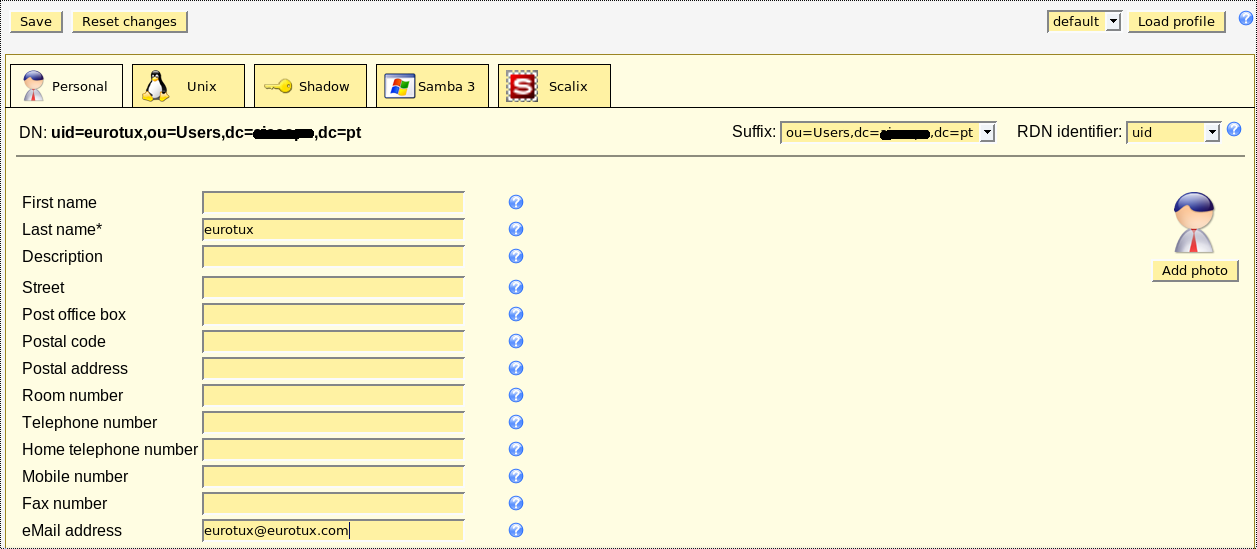
\includegraphics[width=10cm]{include/img/lam4}
    \end{center}
    \caption{Edição Utilizador}
    \label{fig:LAM4}
\end{figure}

No menu superior deverá encontrar todas as directivas associadas ao utilizador:

\begin{itemize}
\item Personal - Edição de dados como primeiro e último nome, endereço de email, etc.
\item Unix - Edição de dados como nome do utilizador, número UID, grupo primário, localização da home-directory, mudar a palavra-passe, etc.
\item Shadow - Tempo de vida da password mínimo e máximo, data de expiração.
\item Samba 3 - Definições de acesso windows, nomeadamente data de expiração, drive para a home-directory, etc.
\item Qmail - Definições da conta de correio do utilizador, quota de email, nomes alternativos, etc.
\item Quota - Quota de ficheiros no servidor.
\item Scalix - Definições de conta de correio no caso de ser usado o servidor scalix
\end{itemize}

\subsubsection{Groups}

Neste interface poderá encontrar a listagem de grupos de utilizadores e poderá criar, editar ou remover grupos de utilizadores. Existem alguns grupos previamente criados utilizados pelo sistema mas poderá criar novos grupos de acordo com a estrutura lógica da empresa.

\begin{figure}[H]
    \begin{center}
        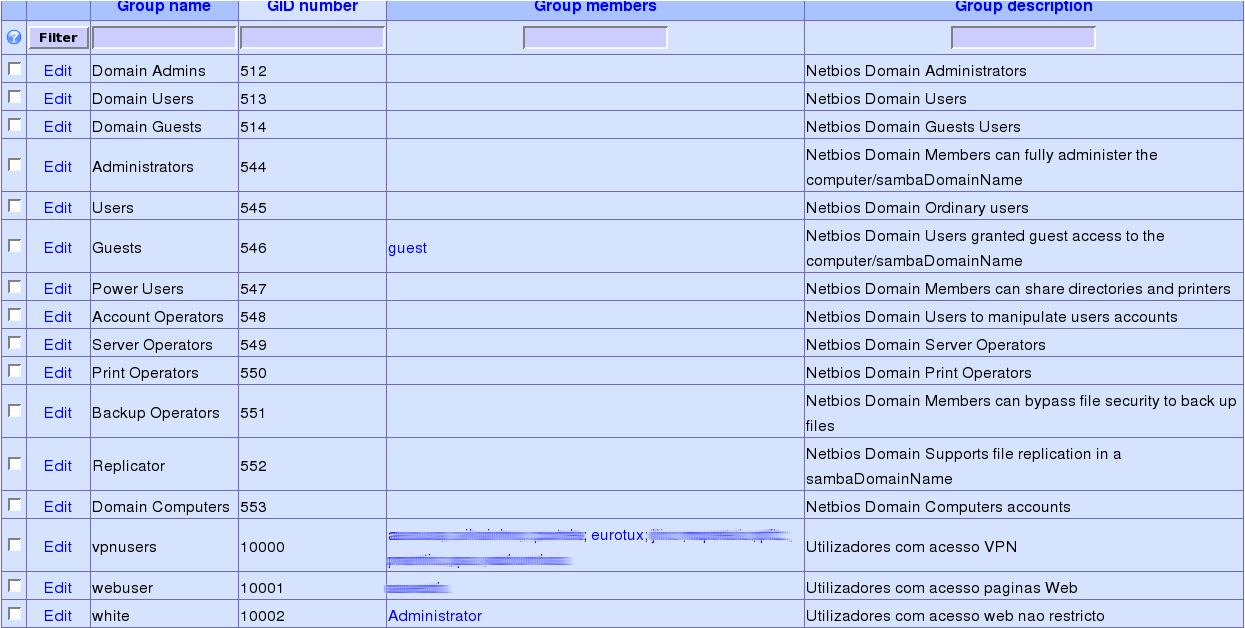
\includegraphics[width=10cm]{include/img/lam6}
    \end{center}
    \caption{Listagem de grupos}
    \label{fig:LAM6}
\end{figure}

\subsubsection{Hosts}

Neste interface poderá encontrar a listagem de postos de computadores que estão inseridos no domínio de samba. Na imagem seguinte poderá encontrar o servidor de domínio bem como um servidor WIN. Poderá, se assim o desejar, remover postos do domínio. Para adicionar novos postos ao domínio deverá ser efectuada a adição no posto em questão.

\begin{figure}[H]
    \begin{center}
        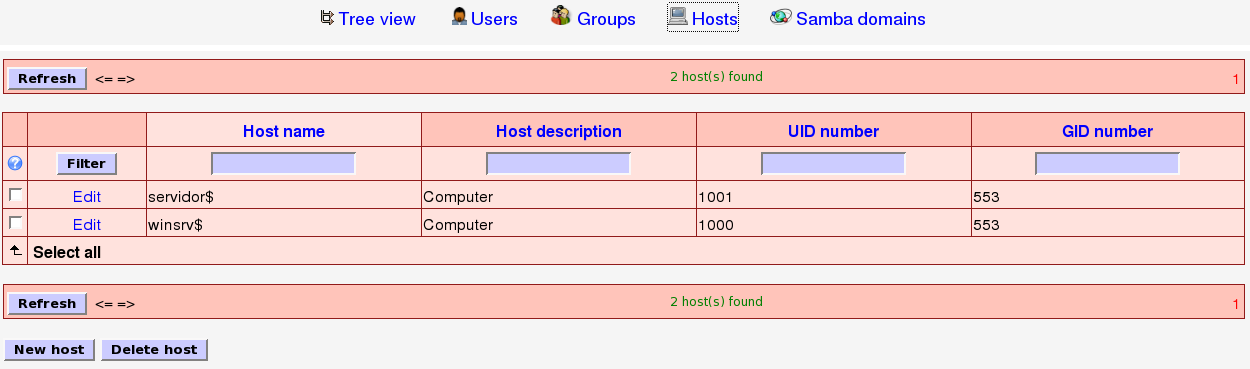
\includegraphics[width=10cm]{include/img/lam7}
    \end{center}
    \caption{Listagem de postos no domínio}
    \label{fig:LAM7}
\end{figure}

\subsubsection{Samba domains}

Neste interface poderá encontrar a listagem dos domínios SMB que estão geridos pelo servidor.

\begin{figure}[H]
    \begin{center}
        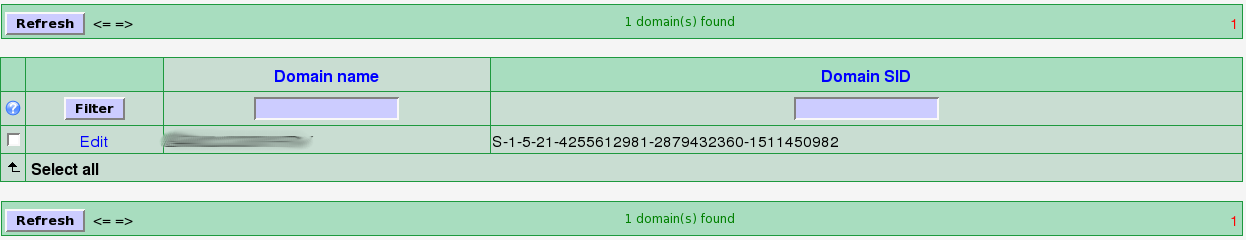
\includegraphics[width=10cm]{include/img/lam8}
    \end{center}
    \caption{Listagem de domínios}
    \label{fig:LAM8}
\end{figure}

\subsection{Criação de um utilizador}
De seguida vamos seguir os passos necessários para criar um novo utilizador. Para tal deverá escolher no menu superior o link "Users". Posteriormente deverá aparecer-lhe uma página com a listagem dos utilizadores. No final dessa listagem aparece um botão "New user". Quando carregar nesse botão deverá aparecer uma página semelhante à seguinte:

\begin{figure}[H]
    \begin{center}
        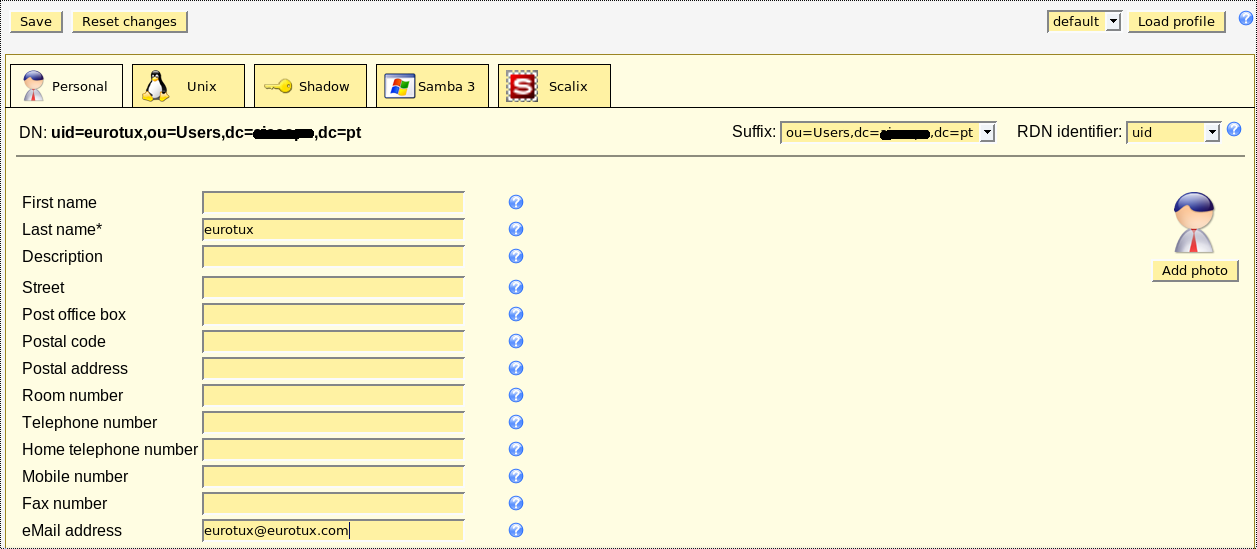
\includegraphics[width=10cm]{include/img/lam4}
    \end{center}
    \caption{Criação de um novo utilizador - Inicial}
    \label{fig:LAM9}
\end{figure}

Vamos agora preencher os campos do utilizador. Nesta página deverão ser então preenchidos os campos de último nome (lastname) e endereço de e-mail (email) obrigatoriamente. Poderá também preencher outros caso deseje mas não são necessários.

Posteriormente vamos escolher a opção "Unix" no menu. Deverá aparecer uma página semelhante à seguinte onde deverá preencher obrigatoriamente os seguintes campos:

\begin{itemize}
\item User Name - Nome do utilizador (sem caractéres acentuados nem espaços em branco)
\item Common Name - Nome do utilizador
\item UID Number - Deixar em branco. Será gerado automaticamente pelo sistema.
\item Primary Group - Grupo principal ao qual o utilizador pertence. Normalmente escolhe-se "Domain Users"
\item Password - Inserir a palavra-passe do utilizador
\item Repeat Password - Inserir novamente a palavra-passe do utilizador
\item Login Shell - Normalmente escolhe-se "/bin/false"
\end{itemize}

\begin{figure}[H]
    \begin{center}
        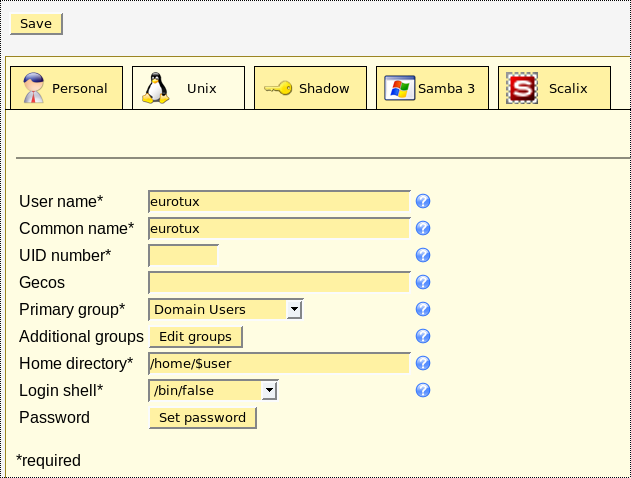
\includegraphics[width=10cm]{include/img/lam10}
    \end{center}
    \caption{Criação de um novo utilizador - Unix}
    \label{fig:LAM10}
\end{figure}

De seguida vamos escolher a opção "Samba" no menu. Devemos carregar em "Add samba3 account".

\begin{figure}[H]
    \begin{center}
        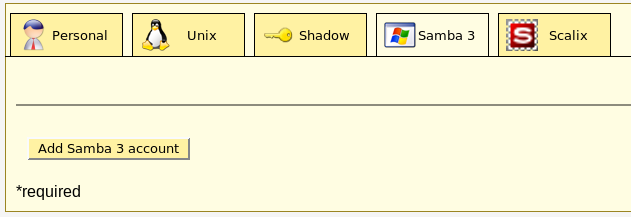
\includegraphics[width=10cm]{include/img/lam9}
    \end{center}
    \caption{Criação de um novo utilizador - SAMBA1}
    \label{fig:LAM9}
\end{figure}



No formulário deverá preencher os seguintes campos:

\begin{itemize}
\item Samba password - Inserir a palavra-passe inserida anteriormente.
\item Repeat password - Inserir novamente a palavra-passe do utilizador.
\end{itemize}

\begin{figure}[H]
    \begin{center}
        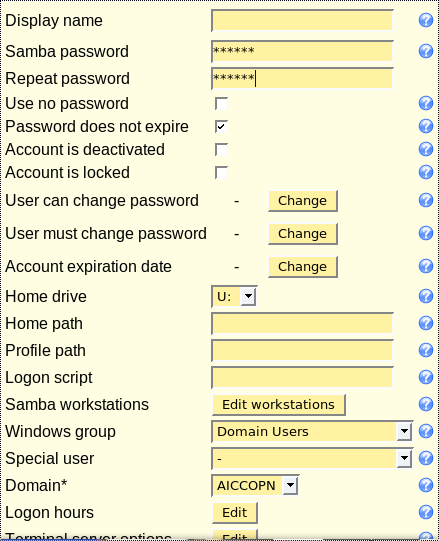
\includegraphics[width=10cm]{include/img/lam11}
    \end{center}
    \caption{Criação de um novo utilizador - Samba}
    \label{fig:LAM11}
\end{figure}

De seguida vamos escolher a opção "Qmail" no menu (esta opção só deverá aparecer se tiver instalado um servidor de mail QMAIL). No formulário poderá preencher os seguintes campos:

\begin{itemize}
\item Mail quota - Tamanho máximo da caixa de correio
\item Allow relay - Permite que o utilizador envie emails para o exterior da organização.
\item Account is activated - A conta de email está activada.
\item Email Aliases - Endereços adicionais para a mesma conta de correio
\end{itemize}

\begin{figure}[H]
    \begin{center}
        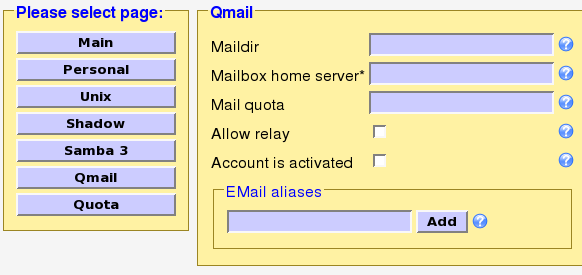
\includegraphics[width=10cm]{include/img/lam12}
    \end{center}
    \caption{Criação de um novo utilizador - Qmail}
    \label{fig:LAM12}
\end{figure}

Se desejar definir a quota de ficheiros no sistema deverá no menu escolher a opção "Quota" onde deverá encontrar uma página semelhante à seguinte (esta opção só aparecerá caso tenha sido activada):

\begin{figure}[H]
    \begin{center}
        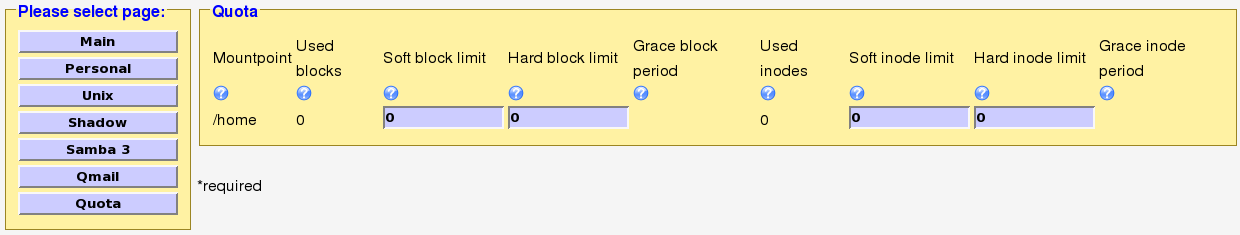
\includegraphics[width=10cm]{include/img/lam13}
    \end{center}
    \caption{Criação de um novo utilizador - Quota}
    \label{fig:LAM13}
\end{figure}

Nas duas primeiras caixas poderá indicar o tamanho máximo (em bytes) de ficheiros. A caixa "Soft block limit" define um limite de aviso enquanto eu a caixa "Hard block limit" define o limite maximo.

No caso de ter um sistema de email scalix deverá ir no menu à opção "Scalix" onde deverá encontrar uma página semelhante à seguinte:

\begin{figure}[H]
    \begin{center}
        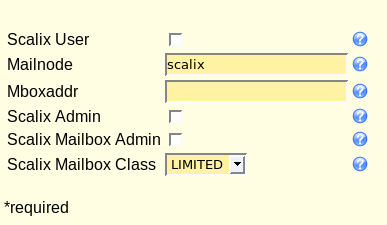
\includegraphics[width=10cm]{include/img/lam14}
    \end{center}
    \caption{Criação de um novo utilizador - Scalix}
    \label{fig:LAM14}
\end{figure}

No formulário poderá preencher os seguintes campos:

\begin{itemize}
\item Scalix User - Se se trata de um utilizador de scalix (de email) esta opção deverá ser activada
\item Mailnode - Servidor de scalix onde a conta estará alojada
\item Mboxaddr - Endereço de email (caso não tenha sido definido no menu "Personal")
\item Scalix Admin - Se se trata de um administrador do servidor de email
\item Scalix Mailbox Admin - Se se trata de um administrador de mailboxes
\item Scalix Mailbox Class - Tipo de utilizador (Limitado - não necessita de licenças, Full - necessita de licenças)
\end{itemize}

Agora que já temos todos os parâmetros do novo utilizador definidos, vamos carregar no botão de "Save".

Como poderá ver, agora o botão "Create account" já se encontra activado indicando que já tem as informações necessárias para criar o utilizador. Para finalizar a criação do utilizador deverá carregar nesse botão. Se a operação correr bem deverá ter uma imagem informativa como a seguinte:

\begin{figure}[H]
    \begin{center}
        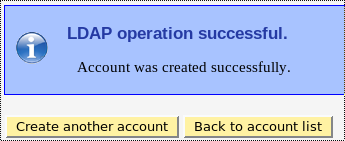
\includegraphics[width=10cm]{include/img/lam15}
    \end{center}
    \caption{Criação de um novo utilizador - Mensagem de sucesso}
    \label{fig:LAM15}
\end{figure}


